\documentclass[]{article}

\usepackage{graphicx}

\title{Acta Fundacional}
\date{}

\begin{document}

\maketitle

Este acta funcional establece de manera clara y sintética cuales van a ser los acuerdos que van a regir el funcionamiento del equipo.

\textbf{Reunidos el día 28 de octubre de 2020}, a las 11:00 horas, las personas que a continuación se detallan:

\begin{enumerate}

\item{Alonso Díez, Jaime, con DNI 32092645-D}
\item{Fuentes Gómez, Alejandro con DNI 29502991-V}
\item{Moreno Olmo, Miguel Ángel con DNI 53964225-S}
\item{Muñoz Ramírez, Víctor con DNI 47566209-R}
\item{Pardo Pastor, Carlos con DNI 47563095-S}
\item{Reina Gutiérrez, Enrique con DNI 29502713-S}

\end{enumerate}

\textbf{Acuerdan:}

\begin{enumerate}
	\item{Finalizar las tareas asignadas dentro de las fechas establecidas por el equipo.}
	\item{Todos los miembros deben de realizar aproximadamente el mismo número de puntos de historia de usuario en cada sprint.}
	\item{Acudir al 80\% de las reuniones programadas para cada sprint.}
	\item{No faltar el respeto a ninguno de los demás miembros del equipo.}
	\item{No mantenerse incomunicado por más de 1 día entero sin 	justificación.}
	\item{No criticar el trabajo de otro a las espaldas, sino hablar de ello directamente en una reunión y de forma constructiva.}
	\item{No negarse a hacer cualquier trabajo asignado en equipo.}
	\item{No mentir sobre su trabajo realizado.}
	\item{Siempre incluir las referencias de cualquier material externo introducido en el proyecto.}
	
	\clearpage
	\item{Respetar la estructura organizativa del equipo:}
	
	\begin{itemize}
	
		\item{Jefe de Proyecto: Enrique Reina Gutiérrez}
		\item{Secretario: Alejandro Fuentes Gómez}
		\item{Equipo de coordinación:}
			
		\begin{itemize}
	
			\item{Miguel Ángel Moreno Olmo}
			\item{Enrique Reina Gutiérrez}
			
		\end{itemize}
		
		\item{Equipo de desarrollo:}
			
		\begin{itemize}
	
			\item{Jaime Alonso Díez}
			\item{Víctor Muñoz Ramírez}
			\item{Carlos Pardo Pastor}
			
		\end{itemize}
		
	\end{itemize}
	
	\begin{center}

	\textit{*Jefe de Proyecto, Secretario y Equipo de coordinación no son roles excluyentes del Equipo de Desarrollo.}

	\end{center}
	
	\item{No realizar trabajo sin informar previamente de ello al equipo.}
	
	\item{La metodología de trabajo será como se indica a continuación:}
	
En primer lugar, el grupo de trabajo va a hacer uso de metodología ágil, concretamente se va a hacer uso de Scrum. Consecuentemente, acorde a la metodología Scrum, se detallará el completo de tareas a realizar, confeccionando el “product backlog”. Para el desarrollo del proyecto, las tareas a realizar se dividirán en diferentes sprints, es decir, para cada sprint se realiza el “sprint backlog”. Con respecto a la duración de cada sprint, se ha acordado que sea de una semana.

A la hora de división del trabajo las tareas del sprint backlog serán divididas entre los integrantes según las cualidades que tenga, se intentará que cada uno de los integrantes realice la misma carga de trabajo que será establecido mediante un Scrum Póker para que cada uno de los integrantes haga los mismos puntos de historia.

Durante el desarrollo de un sprint, el equipo de trabajo va a realizar dos reuniones ordinarias de seguimiento del proyecto. Al terminar el sprint, el equipo de trabajo se dispone a revisar el contenido terminado del sprint, es decir, completar una “sprint review”. Al terminar dicha revisión, el equipo de trabajo realiza una reunión para comentar el funcionamiento del equipo, es decir, realiza una “sprint retrospective”.

\end{enumerate}

\clearpage

En caso de que alguno de los miembros del equipo no cumplan el acuerdo, se aplicarán las siguientes sanciones, las cuales se divide en tres niveles:

\begin{enumerate}

	\item{Sanción Leve: Se le da al sancionado un aviso verbal justificando el por qué de esa sanción.}
	\item{Sanción Media: Además de una sanción leve, se le penaliza con una disminución de horas de trabajo realizadas y sanción escrita que registre la incidencia.}
	\item{Sanción Grave: Se acudirá al coordinador de la asignatura para que trate resolver el conflicto.}
	\item{Sanción Última: Se expulsa al miembro del equipo y se le presenta al coordinador un acta firmada por todos los integrantes que consensuan esa decisión.}

\end{enumerate}

Cada vez que se incumpla un acuerdo, el nivel de sanción será incrementado, por ende, a la cuarta sanción, el causante será expulsado.

Para el caso de discrepancias ante una decisión del trabajo, no existe penalización, pero se debe acudir al resto del equipo.

\clearpage

Y sin más acuerdos que tratar se levanta la sesión, siendo las \textbf{11:30 horas del día 28 de octubre de 2020}:

\begin{table}[!htb]
\begin{tabular}{ c c }


\includegraphics[scale=0.75]{Firmas/Jaime}
& 

\includegraphics[scale=1]{Firmas/Alejandro} \\


Fdo.: Alonso Díez,  Jaime
&
Fdo.: Fuentes Gómez, Alejandro \\

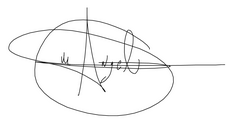
\includegraphics[scale=0.75]{Firmas/MiguelAngel}
&

\includegraphics[scale=0.75]{Firmas/Victor} \\

Fdo.: Moreno Olmo, Miguel Ángel
&
Fdo.: Muñoz Ramírez, Víctor \\


\includegraphics[scale=0.75]{Firmas/Carlos}
&

\includegraphics[scale=0.75]{Firmas/Enrique} \\

Fdo.: Pardo Pastor, Carlos
&
Fdo.: Reina Gutiérrez, Enrique

\end{tabular}
\end{table}

\end{document}